%
% $Id: comb.tex 14 2014-02-04 22:36:30Z nicb $
%
\svnInfo $Id: comb.tex 14 2014-02-04 22:36:30Z nicb $

\chapter{Filtri a pettine (Comb)\label{chap:comb}}

Quando abbiamo studiato i filtri FIR (cf. Cap.\ref{chap:fir}) abbiamo
visto che si possono realizzare filtri nella forma

\begin{equation}\label{eq:invcomb}
  y_t = x_t - R^{L} x_{t-L}
\end{equation}

dove $y$ e $x$ sono, come di consueto, rispettivamente la nostra uscita e il
nostro ingresso. Questi filtri erano costituiti dalla somma algebrica
dell'ingresso e della sua copia ritardata di $L$ campioni.

Se sostituiamo all'ingresso ritardato \emph{l'uscita} ritardata, otteniamo

\begin{equation}
  y_t = x_t + R^{L} y_{t-L}
\end{equation}

La rappresentazione vettoriale di questa equazione \`e

\begin{equation}
  Y = X + R^{L} z^{-L} Y
\end{equation}

Se raggruppo i fattori ottengo

\begin{equation}
  Y - R^{L} z^{-L} Y = Y ( 1 - R^{L} z^{-L} ) = X
\end{equation}

ossia

\begin{equation}
  Y = \frac{X}{1 - R^{L} z^{-L}}
\end{equation}

Quindi la funzione di trasferimento \`e

\begin{equation}
 H ( z ) = \frac{1}{1 - R^{L} z^{-L}}
\end{equation}

Un filtro con questa funzione di trasferimento si chiama
\emph{filtro a pettine}.

Questa funzione di trasferimento \`e il reciproco della funzione di
trasferimento dell'equazione \ref{eq:invcomb}. Quindi se li mettiamo in 
cascata otteniamo una risposta unitaria perch\'e l'azione del primo
canceller\`a quella del secondo.
Per constatare questo basta metterli uno dietro l'altro:

\begin{equation}
  \begin{array}{r c r c l}
	  y_t & = & x_t & - & R^{L} x_{t-L}\\
		w_t & = & y_t & + & R^{L} w_{t-L}\\
	\end{array}
\end{equation}

($w_t$ \`e l'uscita ottenuta usando l'uscita del primo filtro, $y_t$, come
ingresso del secondo filtro).

Ma

\begin{equation}
  y_t = w_t - R^{L} w_{t-L}
\end{equation}

Se sostituisco $y_t$ nella prima equazione ottengo

\begin{equation}
	x_t - R^{L} x_{t-L} = w_t - R^{L} w_{t-L}
\end{equation}

Se il segnale \`e causale, noteremo che $x_t = w_t$
per $t = 0, 1, \dots , L - 1$ dato che $x_{t - L}$ e $w_{t - L}$
valgono zero in quell'ambito.
Applicando lo stesso ragionamento potremo osservare che
$x_t = w_t$ per $t = L, L + 1, \dots, 2 L - 1$. E cos\`i via a blocchi di $L$
campioni. Quindi evidentemente si tratta dello stesso segnale spostato di $L$
campioni.

\begin{figure}[htbp]
	\begin{center}
	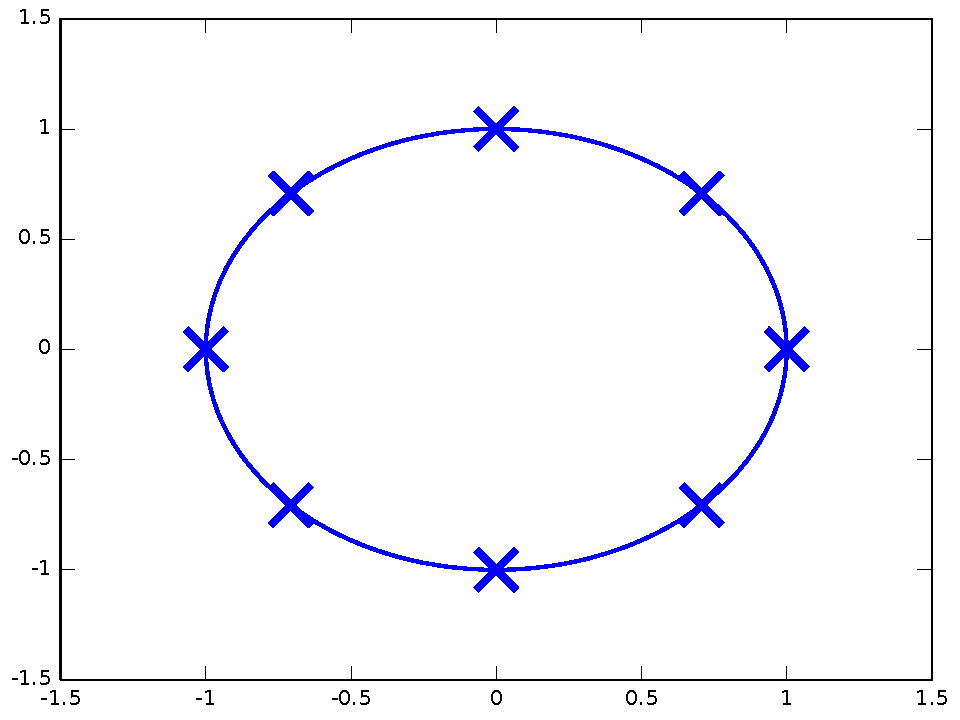
\includegraphics[width=0.75\textwidth]{\plotdir/comb_2}
	\caption{La collocazione dei poli in un filtro comb di ottavo ordine con
	fattore $R = 0.999999$\label{fig:comb poles}}
	\end{center}
\end{figure}

\begin{figure}[htbp]
	\begin{center}
	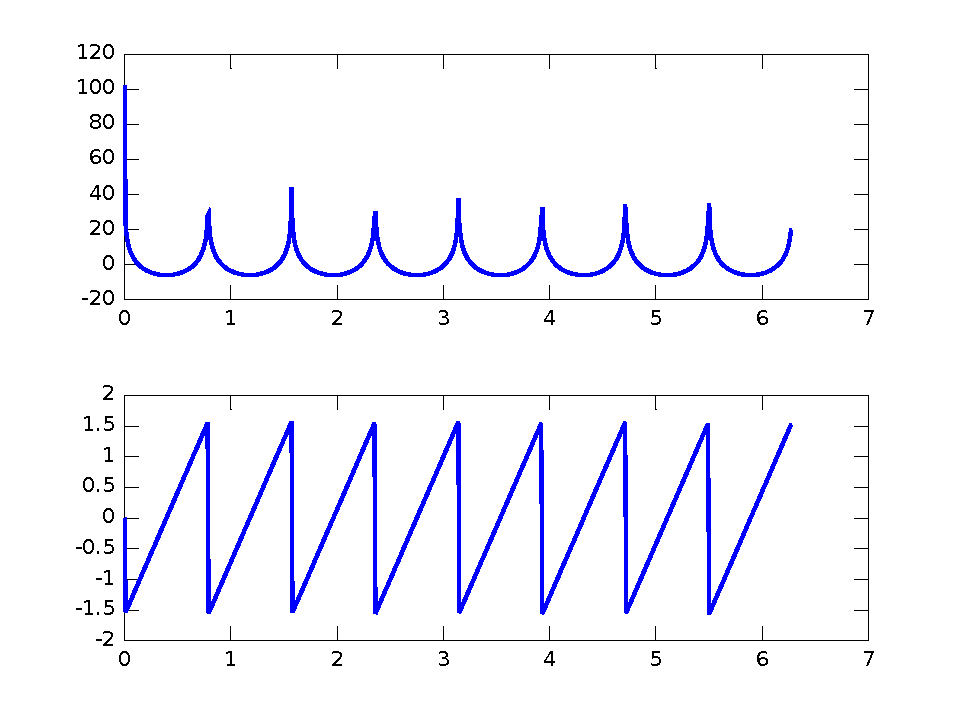
\includegraphics[width=0.75\textwidth]{\plotdir/comb_1}
	\caption{Magnitudine e fase di un filtro comb di ottavo ordine con
	fattore $R = 0.999999$\label{fig:comb magnitude and phase}}
	\end{center}
\end{figure}

\begin{figure}[htbp]
	\begin{center}
	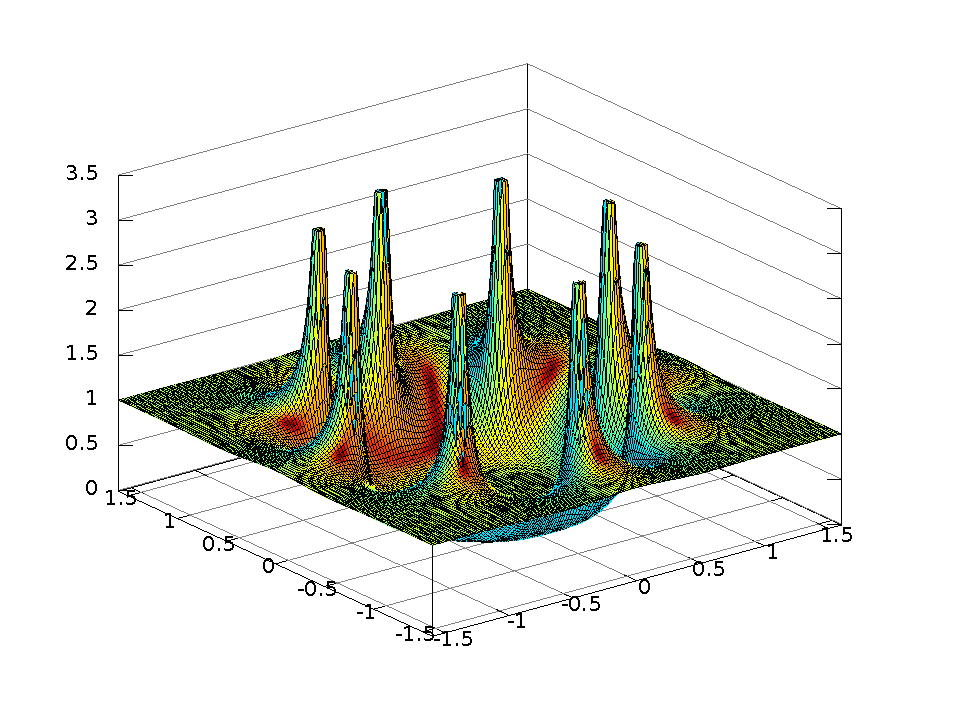
\includegraphics[width=0.75\textwidth]{\plotdir/comb_3}
	\caption{Magnitudine di un filtro comb di ottavo ordine con
	fattore $R = 0.999999$ sul piano zeta\label{fig:comb z-plane poles}}
	\end{center}
\end{figure}

\section{Implementazione \emph{real--world}}

Nel mondo reale i filtri a pettine vengono usati per diversi effetti in campo
audio e musicale. La fig.\vref{fig: real world comb} illustra la risposta
all'impulso di un filtro comb con frequenza di risonanza $233 Hz$, ossia con
un ritardo di 189 campioni.
\begin{figure}[htbp]
	\begin{center}
	  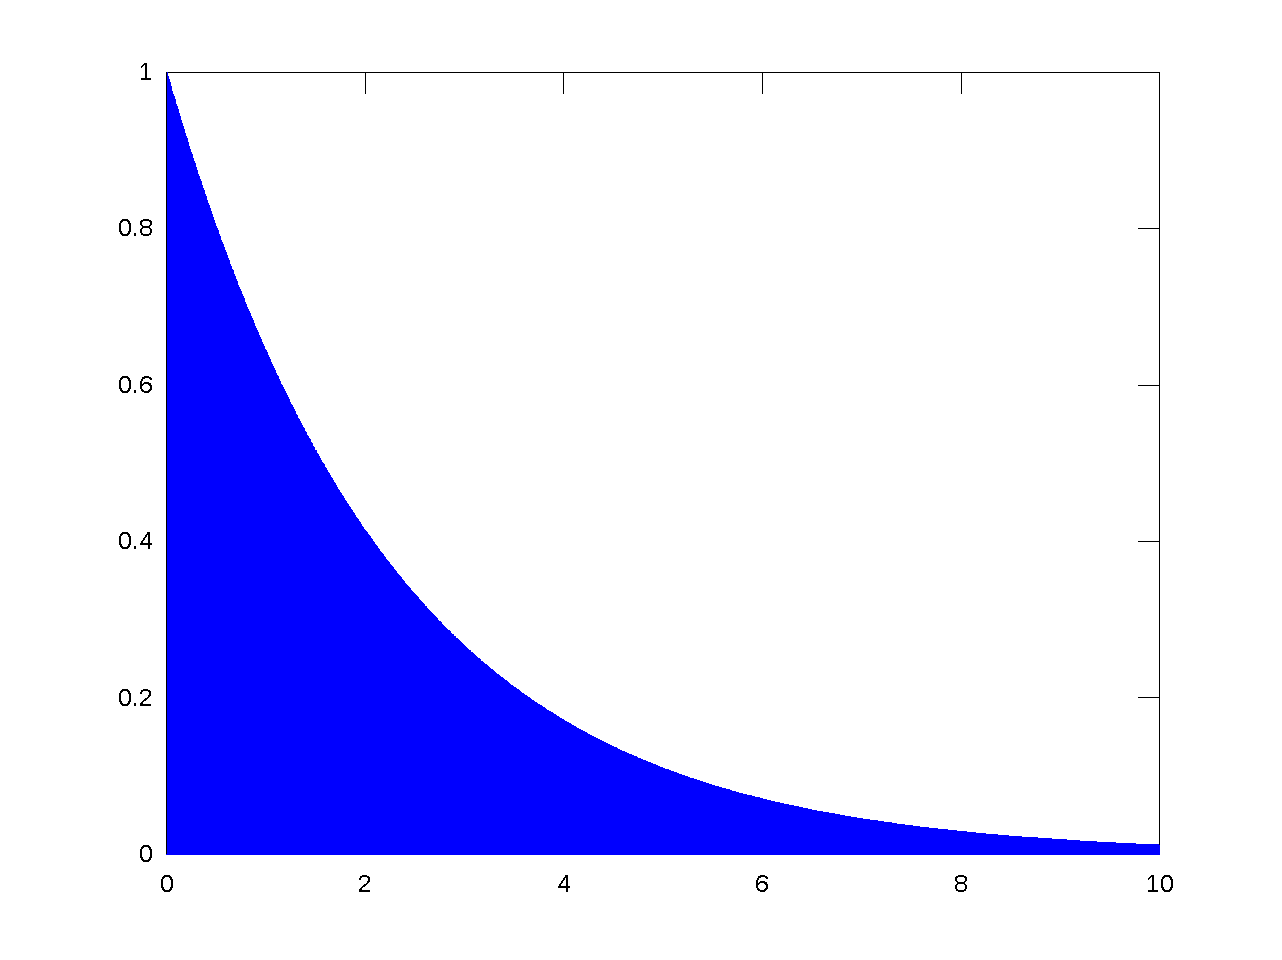
\includegraphics[width=0.75\textwidth]{\plotdir/comb_real}
	  \caption{Risposta all'impulso di un filtro a pettine con frequenza di
		risonanza $233 Hz$\label{fig: real world comb}}
	\end{center}
\end{figure}

\section{Analogia con le onde stazionarie}

Riflettendoci sopra, i filtri comb altro non fanno che aggiungere l'uscita
attenuata e ritadata di $L$ campioni all'ingresso. E` il meccanismo
dell'\emph{eco}.

C'\`e anche una robusta analogia con la riflessione delle onde stazionarie,
ad esempio in un tubo con entrambi le estremit\`a chiuse (o con entrambi le
estremit\`a aperte): le estremit\`a chiuse cambiano di segno alla riflessione
mentre le estremit\`a aperte no. Le altre onde che si propagano in questo modo
sono quelle delle corde tenute ferme ad entrambe le estremit\`a.
